\documentclass[11pt]{exam}
\usepackage[utf8]{inputenc}
\usepackage[a4paper,top=2cm,left=2cm,right=2cm,bottom=2cm]{geometry}
\usepackage{import}
\usepackage[T1]{fontenc}
\usepackage[german,ngerman]{babel}
\usepackage[table]{xcolor}
\usepackage{amsthm, esvect}
\usepackage{mathtools}
\RequirePackage{amssymb, amsfonts, amsmath, latexsym, verbatim, xspace}
\usepackage{systeme}
\usepackage{multicol}
\usepackage{multirow}
\usepackage{framed}
\usepackage{array}
\usepackage{ragged2e}
\usepackage{graphicx}
\usepackage{pdflscape}
\usepackage{epstopdf}
\usepackage{booktabs}
\usepackage{pdfpages}
\usepackage{float} % Allows putting an [H] in \begin{figure} to specify the exact location of the figure
\usepackage{wrapfig} % Allows in-line images such as the example fish picture
\usepackage{tikz, graphicx} % tikz
\usepackage[position=top]{subfig}
\usepackage[bookmarks=true]{hyperref}%Links
\usepackage{enumerate}
\usepackage{enumitem}
\usepackage[german,ruled,vlined,linesnumbered,algosection]{algorithm2e}
\usepackage[labelfont=sf]{caption}
\usepackage{lmodern}
\usepackage{lscape}
\usepackage{tabularx}
\usepackage{systeme}
\usepackage{hhline}
\usepackage{subfiles}
\usepackage{stackengine}
\usepackage{setspace}
\usepackage{MnSymbol}
\usepackage{tcolorbox}
\usepackage{bbm}
\usepackage{url}
\usepackage{xparse}
\usepackage{sectsty}
\usepackage{array}
\usepackage{ragged2e}
\usepackage{listings} %Stellt Code-Snippets sauber dar

% definiert die Sprache
\selectlanguage{German}

% add command for different dates in Swiss fashion
\newcommand{\monthwordlong}[1]{\ifcase#1 \or Januar\or Februar\or März\or April\or Mai\or Juni\or Juli\or August\or September\or Oktober\or November\or Dezember\fi}
\newcommand{\monthwordshort}[1]{\ifcase#1\or Jan\or Feb\or Mar\or Apr\or Mai\or Jun\or Jul\or Aug\or Sept\or Okt\or Nov\or Dez\fi}
\newcommand{\datelong}{\number\day.\:\monthwordlong{\the\month}\:\number\year}
\newcommand{\dateshort}{\number\day.\:\monthwordshort{\the\month}\:\number\year}

% define color of links inside a text
\definecolor{linkblue}{RGB}{0, 0, 80}
\definecolor{plotblue}{RGB}{100, 100, 255}
\definecolor{myblue}{RGB}{8,164,214}
\definecolor{myred}{RGB}{143,42,41}
\definecolor{forestgreen}{RGB}{34,139,34}
\definecolor{highdive}{RGB}{10,169,194}
\definecolor{charcoal}{RGB}{74,74,74}
\hypersetup{
	colorlinks=true,
	linkcolor=linkblue,
	filecolor=magenta,
	urlcolor=plotblue,
	citecolor=linkblue,
	pdfpagemode=FullScreen,
}


\lstdefinestyle{mystyle}{ % definiert den style des Code-Snippets
	%backgroundcolor=\color{backcolour},
	%commentstyle=\color{codegreen},
	%keywordstyle=\color{magenta},
	%numberstyle=\tiny\color{codegray},
	%stringstyle=\color{codepurple},
	basicstyle=\ttfamily\footnotesize,
	breakatwhitespace=false,
	breaklines=true,
	captionpos=b,
	keepspaces=true,
	%numbers=left,
	%numbersep=5pt,
	showspaces=false,
	showstringspaces=false,
	showtabs=false,
	tabsize=4
}
\lstset{style=mystyle}
\qformat{\Large\textbf{Aufgabe \thequestion\hfill\thepoints}}
\newlist{partes}{enumerate}{3}
\setlist[partes]{label=(\alph*)}
\newcommand{\parte}{\item}
\newlist{subpartes}{enumerate}{3}
\setlist[subpartes]{label=\roman*)}
\newcommand{\subparte}{\item}
\setlist[enumerate,1]{%(
	leftmargin=*, itemsep=12pt, label={\textbf{\arabic*.)}}}
\newcommand\answerbox{%%
	\fbox{\rule{2in}{0pt}\rule[-0.1ex]{0pt}{4ex}}}
\pointpoints{Punkt}{Punkte}
\hqword{Frage:}
\hpword{Mögliche Punkte:}
\hsword{Erreicht:}
\htword{Total}
\renewcommand*\half{.5}
\renewcommand{\solutiontitle}{\noindent\textbf{Lösung:}\par\noindent}

% Graphed boxes
\newcommand{\karos}[2]{
  \begin{tikzpicture}
    \draw[step=0.4cm,color=cyan,dotted] (0,0) grid (#1 cm ,#2 cm);
  %  \draw((#1)/2 cm,0)--((#1)/2 cm,/#2)/2cm)
  \end{tikzpicture}
}
\usetikzlibrary{arrows, petri, topaths, graphs}
\linespread{1.2} % Line spacing

%=========================================================
\newenvironment{parcols}[1][]{
    \begin{parts}\begin{multicols}{#1}
}{
    \end{multicols}\end{parts}
}
%=========================================================
\newenvironment{itemcols}[1][]{
	\begin{itemize}\begin{multicols}{#1}
		}{
	\end{multicols}\end{itemize}
}

%=========================================================
\newcommand{\antwort}[1]{
	{\setlength{\textwidth}{\textwidth}\fillwithgrid{#1cm}\vspace{5pt}}
}

%=========================================================
% Karriertes Papier für Antwort MIT OVERLAY
\tcbuselibrary{breakable,skins}
\usetikzlibrary{mindmap,trees}
\newlength\tindent
\setlength{\tindent}{\parindent}
\setlength{\parindent}{0pt}
\setlength{\parskip}{0pt}

\newtcolorbox{gridspace}[1]{%
	enhanced,
	breakable,
	blanker,
	boxrule=0pt,
	left=5mm,
	right=5mm,
	top=5.75mm,
	bottom=0mm,
	boxsep=0pt,
	height=#1cm,
	width=16cm,
	before upper={
		\begingroup
		\setlength{\baselineskip}{5.75mm}
		\setlength{\parskip}{0pt}
		\setlength{\lineskip}{0pt}
		% keep every paragraph on the grid rhythm
		%\everypar{\vspace{0pt}\strut}
		% math formulas shifted by one grid row
		\let\oldbracketopen\[
		\renewcommand{\[}{\vspace{-5mm}\oldbracketopen}
		% Align displayed formulas to the grid
		\setlength{\abovedisplayskip}{0pt}
		\setlength{\belowdisplayskip}{0pt}
		\setlength{\abovedisplayshortskip}{0pt}
		\setlength{\belowdisplayshortskip}{0pt}
		% Enumerate follows the same rhythm
		\setlist[enumerate]{leftmargin=6mm,itemsep=0mm,topsep=0pt,parsep=0pt,partopsep=0pt}
		\setlist[itemize]{leftmargin=6mm,itemsep=10mm,topsep=0pt,parsep=0pt,partopsep=0pt}},
	after upper={
		\endgroup},
	underlay={
		\draw[step=5mm,color=gray!55] (interior.south west) grid (interior.north east);}
}

\pagestyle{headandfoot}
\firstpageheader{}{}{\teacher}
\runningheader{}{}{\teacher}
\firstpagefooter{}{}{Seite \thepage\:von \numpages}
\runningfooter{}{}{Seite \thepage\:von \numpages}
%%
% Math Arrows
%%
\newcommand{\same}{\ensuremath{\Longleftrightarrow}}
\renewcommand{\to}{\ensuremath{\longrightarrow}}
\newcommand{\qsame}{\quad\same\quad}
\newcommand{\dsame}{\ensuremath{:\Leftrightarrow}}
\newcommand{\qdsame}{\quad\dsame\quad}
\newcommand{\ldsame}{\ensuremath{:\Longleftrightarrow}}
\newcommand{\samedef}{\ensuremath{\us {\text{def}} \Leftrightarrow}}
\newcommand{\qsamedef}{\quad\samedef\quad}
\newcommand{\lsamedef}{\ensuremath{\us {\text{def}} \Longleftrightarrow}}
\newcommand{\qlsamedef}{\quad\lsamedef\quad}


%%
% Mengendefinitionen
%%
\newcommand{\M}{\ensuremath{\mathcal{M}}}
\newcommand{\N}{\ensuremath{\mathbb{N}}}
\newcommand{\Z}{\ensuremath{\mathbb{Z}}}
\newcommand{\Q}{\ensuremath{\mathbb{Q}}}
\newcommand{\I}{\ensuremath{\mathbb{I}}}
\newcommand{\R}{\ensuremath{\mathbb{R}}}
\newcommand{\C}{\ensuremath{\mathbb{C}}}
\renewcommand{\S}{\ensuremath{\mathbb{S}}}
\newcommand{\Prim}{\ensuremath{\mathbb{P}}}
\newcommand{\0}{\ensuremath{\emptyset}}
\renewcommand{\Re}{\ensuremath{\operatorname{Re}}}
\renewcommand{\Im}{\ensuremath{\operatorname{Im}}}
\newcommand{\strich}{\ensuremath{\big\vert}}

%%
% Mengenoperation
%%
\renewcommand{\nin}{\not\in}


%%
% Logisches Und und Oder
%%
\newcommand{\sand}{\ensuremath{\; \land \;}}
\newcommand{\sor}{\ensuremath{\; \lor \;}}
\renewcommand{\*}{\ensuremath{\cdot}}
\newcommand{\oder}{\vee}
\newcommand{\n}{\neg}
\newcommand{\und}{\wedge}


%%
% Bei Integral, Summe,... die Grenzen über bzw.
% unter das Zeichen
%%
\renewcommand{\d}[1]{\ensuremath{\operatorname{d}\!{#1}}}
\newcommand{\Sum}{\sum\limits}
\newcommand{\Prod}{\prod\limits}
\newcommand{\Min}{\min\limits}
\newcommand{\Max}{\max\limits}
\newcommand{\Lim}{\lim\limits}
\newcommand{\Inf}{\inf\limits}
\newcommand{\Sup}{\sup\limits}
\newcommand{\Liminf}{\liminf\limits}
\newcommand{\Limsup}{\limsup\limits}
%\renewcommand{\Cup}{\bigcup\limits}
%\renewcommand{\Cap}{\bigcap\limits}
\newcommand{\Otimes}{\bigotimes\limits}
\newcommand{\Oplus}{\bigoplus\limits}


%%
% Arcus Cotangens, Logarithmus
%%
\let\oldsin\sin
\renewcommand{\sin}[1]{\oldsin{\left(#1\right)}}
\let\oldcos\cos
\renewcommand{\cos}[1]{\oldcos{\left(#1\right)}}
\let\oldtan\tan
\renewcommand{\tan}[1]{\oldtan{\left(#1\right)}}
\let\oldarcsin\arcsin
\renewcommand{\arcsin}[1]{\oldarcsin{\left(#1\right)}}
\let\oldarccos\arccos
\renewcommand{\arccos}[1]{\oldarccos{\left(#1\right)}}
\let\oldarctan\arctan
\renewcommand{\arctan}[1]{\oldarctan{\left(#1\right)}}
\let\oldln\ln
\renewcommand{\ln}[1]{\oldln{\left(#1\right)}}
\newcommand{\Log}[2]{\ensuremath{\operatorname{log}_{#1}\left(#2\right)}}
\newcommand{\e}{\operatorname{e}}
\renewcommand{\exp}[1]{\ensuremath{\operatorname{\e}^{#1}}}


%%
% Griechische Buchstaben
%%
\renewcommand{\epsilon}{\ensuremath{\varepsilon}}
\renewcommand{\phi}{\varphi}
\renewcommand{\l}{\lambda}
\renewcommand{\t}{\tau}


%%
% Bezeichnungen
%%
\newcommand{\Rgn}{\R_{>0}} % R grösser Null
\newcommand{\Rad}{\operatorname{Rad}}   % Radikal
\newcommand{\kgV}{\operatorname{kgV}}   % Kleinster gemeinsame Vielfache
\newcommand{\ggT}{\operatorname{ggT}}   % Grösster gemeinsame Teiler
\newcommand{\winkel}{\sphericalangle}          % Winkelsymbol
\DeclarePairedDelimiter\abs{\lvert}{\rvert} % besserer Betrag
\makeatletter
\let\oldabs\abs
\def\abs{\@ifstar{\oldabs}{\oldabs*}}
\makeatother


%%
% Vektorgeometrie
%%
\renewcommand{\v}[1]{\vv{#1}}       % besserer Pfeil über Buchstaben
\renewcommand{\vec}[2]{\begingroup\renewcommand{\arraystretch}{1}\left(\begin{array}{c} #1 \\ #2 \end{array}\right)\endgroup}   % two dimensional vector
\renewcommand{\Vec}[3]{\begingroup\renewcommand{\arraystretch}{1}\left(\begin{array}{c} #1 \\ #2 \\ #3 \end{array}\right)\endgroup}      % three dimensional vector


%%
% Text
%%
\newcommand*{\Ueq}[1]{\mathrel{\mathop{=}\limits_{\text{#1}}}}
\newcommand*{\Oeq}[1]{\mathrel{\stackrel{\text{#1}}{=}}}
\newcommand{\utext}[2]{\underbrace{#1}_{\substack{#2}}}
\newcommand{\otext}[2]{$\overbrace{\textrm{#1}}^{\textrm{#2}}$}
\newcommand{\lineortext}[1]{\hspace{0,1cm}\underline{\hspace{0.1cm}\hphantom{#1}\hspace{0.1cm}}\hspace{0,1cm}} % Lückentext erstellen
\newcommand{\gap}[1]{\rule{#1 cm}{1pt}}
\graphicspath{{data-algebra/}}
%=========================================================
\newcommand{\theme}{Logarithmus}
\newcommand{\teacher}{Jonas Guler}
%=========================================================
\begin{document}
\fontsize{14}{14}\selectfont
\begin{center}
    \huge\bf\theme
\end{center}

\begin{questions}
%=========================================================
%-------------------TESTFRAGEN
%=========================================================
\noaddpoints
\question[\totalpoints]
\addpoints
\begin{parts}
    \part[2] Beschreibe in eigenen Worten, was ein Logarithmus ist und inwiefern er mit der Exponentialfunktion verbunden ist.
    \part[1] Erkläre einem Laien in zwei Sätzen, den Unterschied zwischen einer Polynomialgleichung und einer Exponentialgleichung. Veranschauliche deine Erklärung mit einem passenden Beispiel.
\end{parts}
\begin{parts}
    \setcounter{partno}{2}
    \part[2] Welcher der folgenden Ausdrücke passt nicht dazu? Begründe deine Antwort.
    \[\Log{4}{2}\quad\Log{10}{0.01}\quad\Log{2}{\frac{1}{8}}\quad\Log{3}{\frac{1}{81}}\]
    \part Welcher der folgenden Ausdrücke passt nicht dazu? Begründe deine Antwort.
    \[\Log{4}{2}\quad\Log{10}{100}\quad\Log{2}{8}\quad\Log{3}{81}\]
\end{parts}

\begin{parts}
    \setcounter{partno}{4}
    \part[4] Löse die folgende Exponentialgleichung ohne Verwendung des Taschenrechners nach $x$ auf.
    \[7^{2x-1}\*343^{3x+5}=49^{2x-1}\]
    \begin{small}
        Bewertung: Lösungen ohne Lösungsweg ergeben keine Punkte.
    \end{small}
\end{parts}
\begin{parts}
    \setcounter{partno}{5}
    \part[4] Löse die folgende Exponentialgleichung ohne Verwendung von \flqq solve\frqq\: nach $x$ auf. \[5^{x+2}\*125^{2-x}=25^x\]
    \begin{small}
        Bewertung: Lösungen ohne Lösungsweg ergeben keine Punkte.
    \end{small}
\end{parts}
\begin{parts}
	\setcounter{partno}{6}
	\part[4] Löse die folgende Exponentialgleichung ohne Verwendung von \flqq solve\frqq\: nach $x$ auf. \[4^{x-7}\*16^{2x+1}=64^{x+2}\]
	\begin{small}
		Bewertung: Lösungen ohne Lösungsweg ergeben keine Punkte.
	\end{small}
\end{parts}
\begin{parts}
	\setcounter{partno}{7}
	\part[4] Löse die folgende Exponentialgleichung ohne Verwendung von \flqq solve\frqq\: nach $x$ auf. \[3^{2x-1}\*\left(\frac{1}{9}\right)^{7-x}=\left(\sqrt[4]{3}\right)^x\]
	\begin{small}
		Bewertung: Lösungen ohne Lösungsweg ergeben keine Punkte.
	\end{small}
\end{parts}


%---------------------------------------------------------
\question[4]
Welche der folgenden Ausdrücke ist wahr? Begründe deine Antwort.
\begin{parcols}[2]
    \part $\Log{10}{11^a}=a$
    \part $\Log{b}{\frac{1}{x}}=-\Log{b}{x}$
    \part $\Log{a}{b}=\frac{\ln{a}}{\ln{b}}$
    \part $\Log{2}{x}+\Log{3}{y}=\Log{2}{x\*y}$
\end{parcols}

\question[4]
Begründe, welche der folgenden Ausdrücke wahr sind und korrigiere die falschen Aussagen.
\begin{parcols}[2]
    \part $\Log{a}{u+v}=\Log{a}{u}+\Log{a}{v}$
    \part $\Log{a}{u-v}=\frac{\Log{a}{u}}{\Log{a}{v}}$
    \part $\Log{2}{x}+\Log{3}{y}=\Log{2}{xy}$
    \part $\Log{a}{b}=\frac{\ln{a}}{\ln{b}}$
\end{parcols}

\question[4]
Begründe, welche der folgenden Ausdrücke wahr sind und korrigiere die falschen Aussagen.
\begin{parcols}[2]
    \part $\Log{a}{u+v}=\Log{a}{u}+\Log{a}{v}$
    \part $\Log{a}{\frac{u}{v}}=\frac{\Log{a}{u}}{\Log{a}{v}}$
    \part $\Log{2}{x}+\Log{3}{y}=\Log{2}{xy}$
    \part $\Log{a}{c\*u}=c\*\Log{a}{u}$
\end{parcols}

\question[4]
In das leere Feld ist jeweils ein Ausdruck so einzufüllen, dass insgesamt eine gültige Aussage entsteht.
\begin{parts}
	\part $\displaystyle\Log{a}{\gap{3}}=2\*\Log{a}{p}-3\*\Log{a}{q}-4\*\Log{a}{r}$\newline
	\part $\displaystyle\Log{a}{\sqrt[3]{q^4}}=\gap{3}\*\Log{a}{q}$\newline
	\part $\displaystyle\Log{a}{a^{-\frac{9}{13}}}=\gap{3}$\newline
	\part $\displaystyle\gap{3}=\frac{3\*\ln{x}}{\ln{4}}$\newline
\end{parts}


%---------------------------------------------------------
\question[6]
Schreibe den folgenden Logarithmus in möglichst viele Summanden aus.
\begin{parcols}[3]
        \part $\Log{a}{5a^2c^3}$
        \part $\Log{a}{\frac{2(p^2+q^2)}{x+y}}$
        \part $\Log{a}{\frac{\sqrt[3]{u}}{a^5}}$
    \end{parcols}

%---------------------------------------------------------
\question[2]
Schreibe den folgenden Logarithmus in möglichst viele Summanden aus.
\[\Log{m}{\frac{m^2\sqrt[3]{m^2\*\sqrt{n^3}}}{m\*\sqrt[6]{n}}}\]

%---------------------------------------------------------
\question[2]
Schreibe den folgenden Logarithmus in möglichst viele Summanden aus. \[\Log{a}{\frac{4\sqrt[3]{x}}{5\sqrt{a^3}}}\]

%---------------------------------------------------------
\question[2]
Schreibe den folgenden Logarithmus in möglichst viele Summanden aus. \[\Log{a}{\frac{a^2\sqrt{x}}{x+y}}\]


%---------------------------------------------------------
\question[6]
Fasse den Term zu einem Logarithmus zusammen und vereinfache so weit wie möglich.
\begin{parts}
    \part $\frac{1}{4}\Log{3}{81}+\frac{1}{3}\Log{2}{8}$
    \part $\Log{a}{b^2}+\Log{a}{c^2}-\Log{a}{b}-\Log{a}{c}$
    \part $\ln{x+1}+\ln{x-1}-\ln{x^2-1}$
\end{parts}

%---------------------------------------------------------
\question[2]
Fasse den Term zu einem Logarithmus zusammen und vereinfache so weit wie möglich.
\[\ln{x+1}+\ln{x-1}-\ln{x^2-1}\]

%---------------------------------------------------------
\question[2]
Fasse den Term zu einem Logarithmus zusammen und vereinfache so weit wie möglich.
\[\frac{1}{2}\*\ln{a^{2n}}-(n+2)\ln{a}\]

%---------------------------------------------------------
\question[2]
Fasse den Term zu einem Logarithmus zusammen und vereinfache so weit wie möglich. \[5\*\ln{x+2}-\frac{1}{5}\*\ln{x-2}-4\*\ln{x+2}-\frac{4}{5}\*\ln{x-2}\]


%---------------------------------------------------------
\question[4]
Löse die folgende Gleichung nach $x$ auf. \[\log{x^3}+2\log{x^2}=7\]


%---------------------------------------------------------
\question[4]
Claudia will diese Gleichung lösen: \[5^x=0.2^{3x}\*\exp{x-1}.\] Sie wendet den natürlichen Logarithmus auf beiden Seiten an und erhält \[x\*\ln{5}=3x\*\ln{0.2}\*(x-1).\] Hat sie alles richtig gemacht?
\begin{itemize}
	\item Falls JA, löse die Gleichung fertig.
	\item Falls NEIN, erkläre den Fehler und löse die Gleichung vollständig korrekt.
\end{itemize}


%---------------------------------------------------------
\question[3]
\begin{minipage}{0.6\linewidth}
    Im Koordinatensystem sind drei Graphen von Logarithmusfunktionen eingezeichnet. Ordne die drei Graphen ihrer Funktionsgleichung zu.
    \begin{parts}\begin{multicols}{2}
        \part $y=\Log{\frac{1}{3}}{x}$
        \part $y=\Log{2}{x-1}$
        \part $y=\Log{2}{x}+2$
        \part $y=\Log{\frac{1}{2}}{x}$
        \part $y=\Log{2}{x+1}$
        \part $y=\Log{2}{x-1}+2$
    \end{multicols}\end{parts}
\end{minipage}
\hfill
\begin{minipage}{0.35\linewidth}
    \centering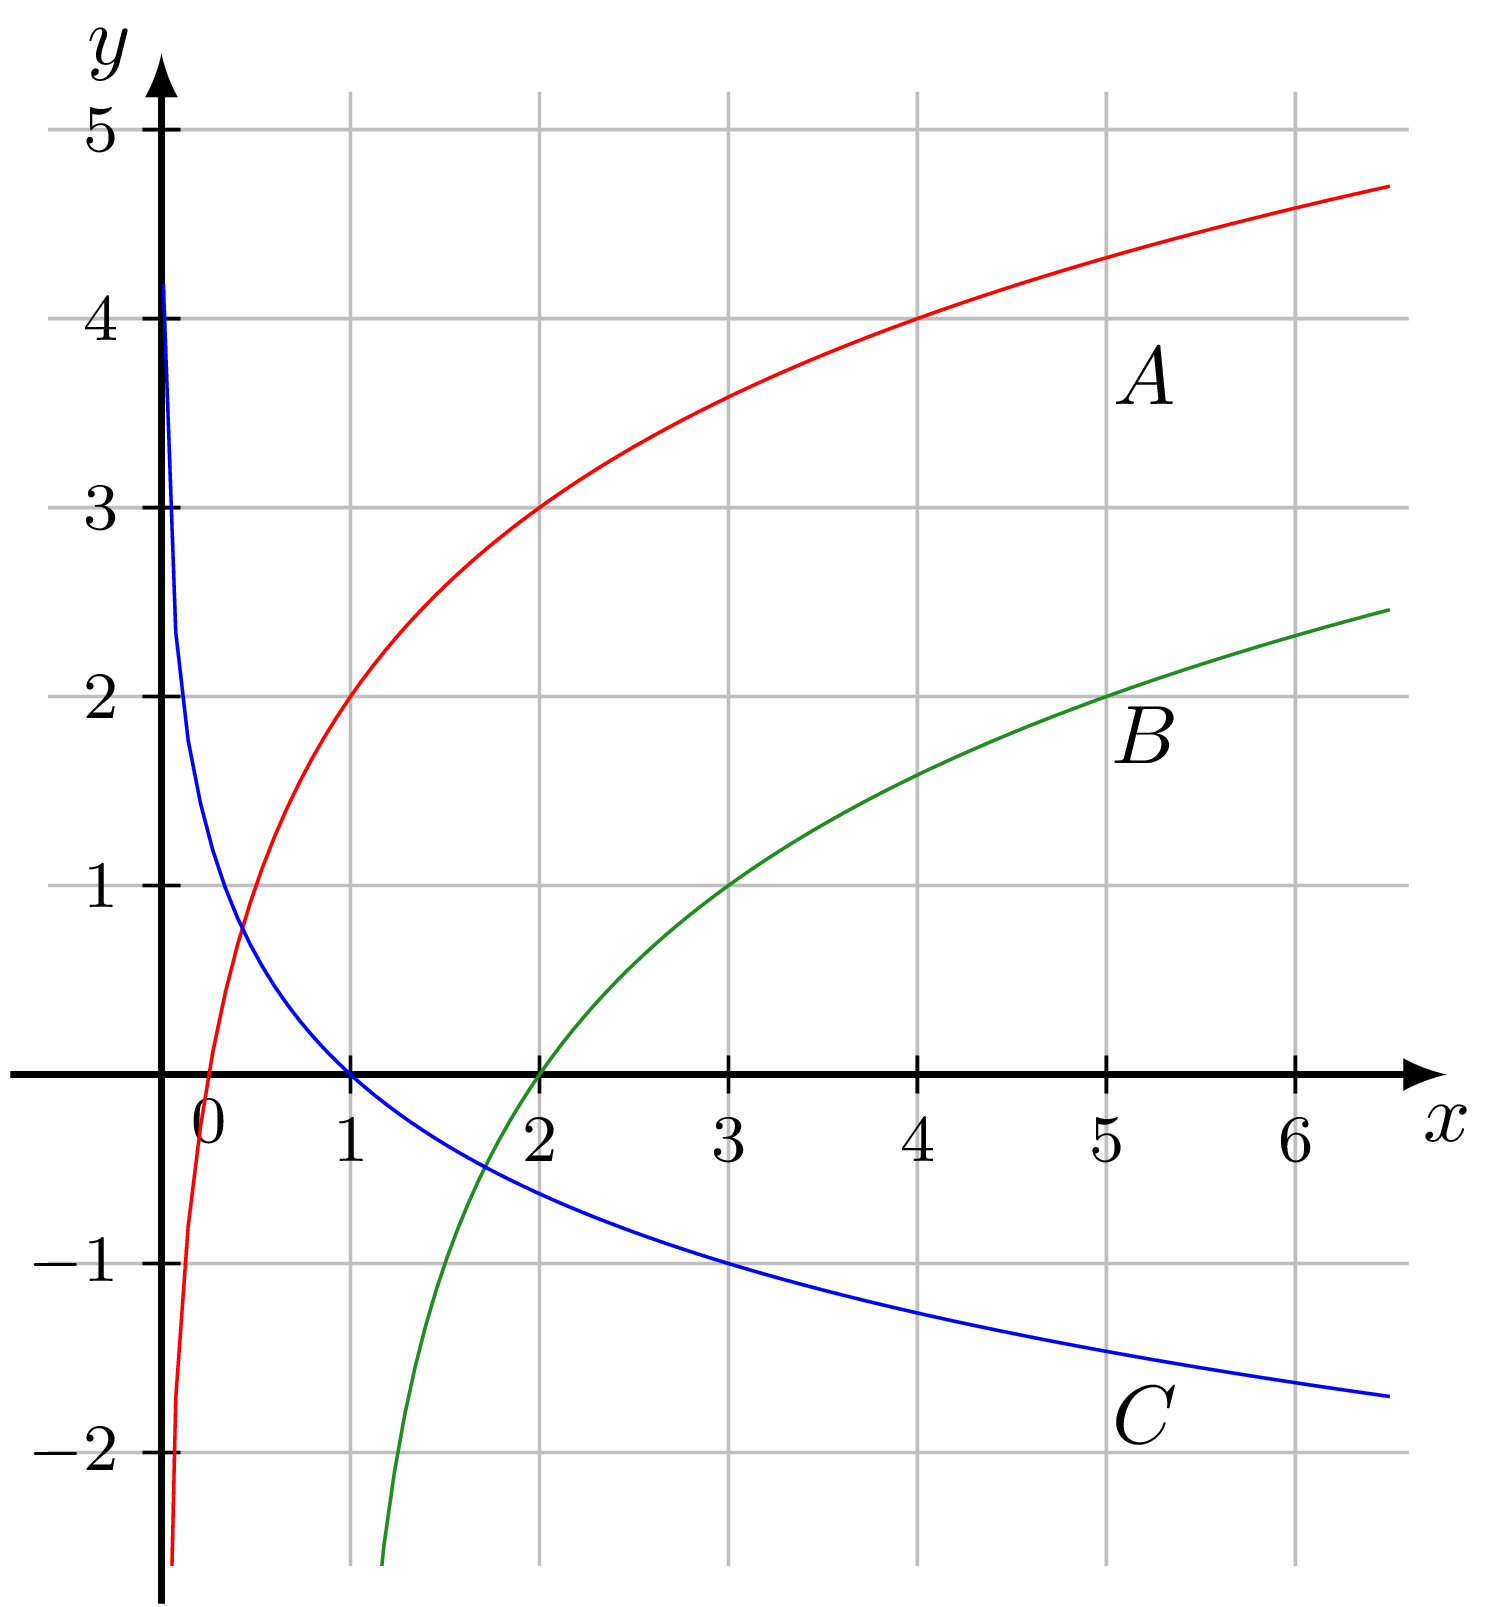
\includegraphics[scale=0.1]{data-algebra/LogGraphen2.png}
\end{minipage}

%---------------------------------------------------------
\question[8]
Berechne die folgenden Logarithmen mithilfe des kleinen Taschenrechner. Notiere deinen Lösungsweg und markiere darin, wo du den Taschenrechner zur Hilfe genommen hast.
\begin{parts}
    \begin{multicols}{2}
        \part $\Log{4}{12}$
        \part $3\cdot\Log{e}{10}$
        \part $\Log{4}{\sqrt{5}}$
        \part $4\cdot\Log{9}{3}$
    \end{multicols}
\end{parts}

%---------------------------------------------------------
\noaddpoints
\question[\totalpoints]
\addpoints
\begin{minipage}{0.6\linewidth}
    \begin{parts}
        \part[2] Gezeichnet sind drei Graphen von Funktionen der Form $y=\Log{b}{x}$. Gib an welcher zur Funktion mit der kleinsten und welcher zur Funktion mit der grössten Basis $b$ gehört.
        \part[1] Gib die Basis der Funktion des Graphen $\textcolor{red}{B}$ an.
    \end{parts}
\end{minipage}
\hfill
\begin{minipage}{0.35\linewidth}
    \centering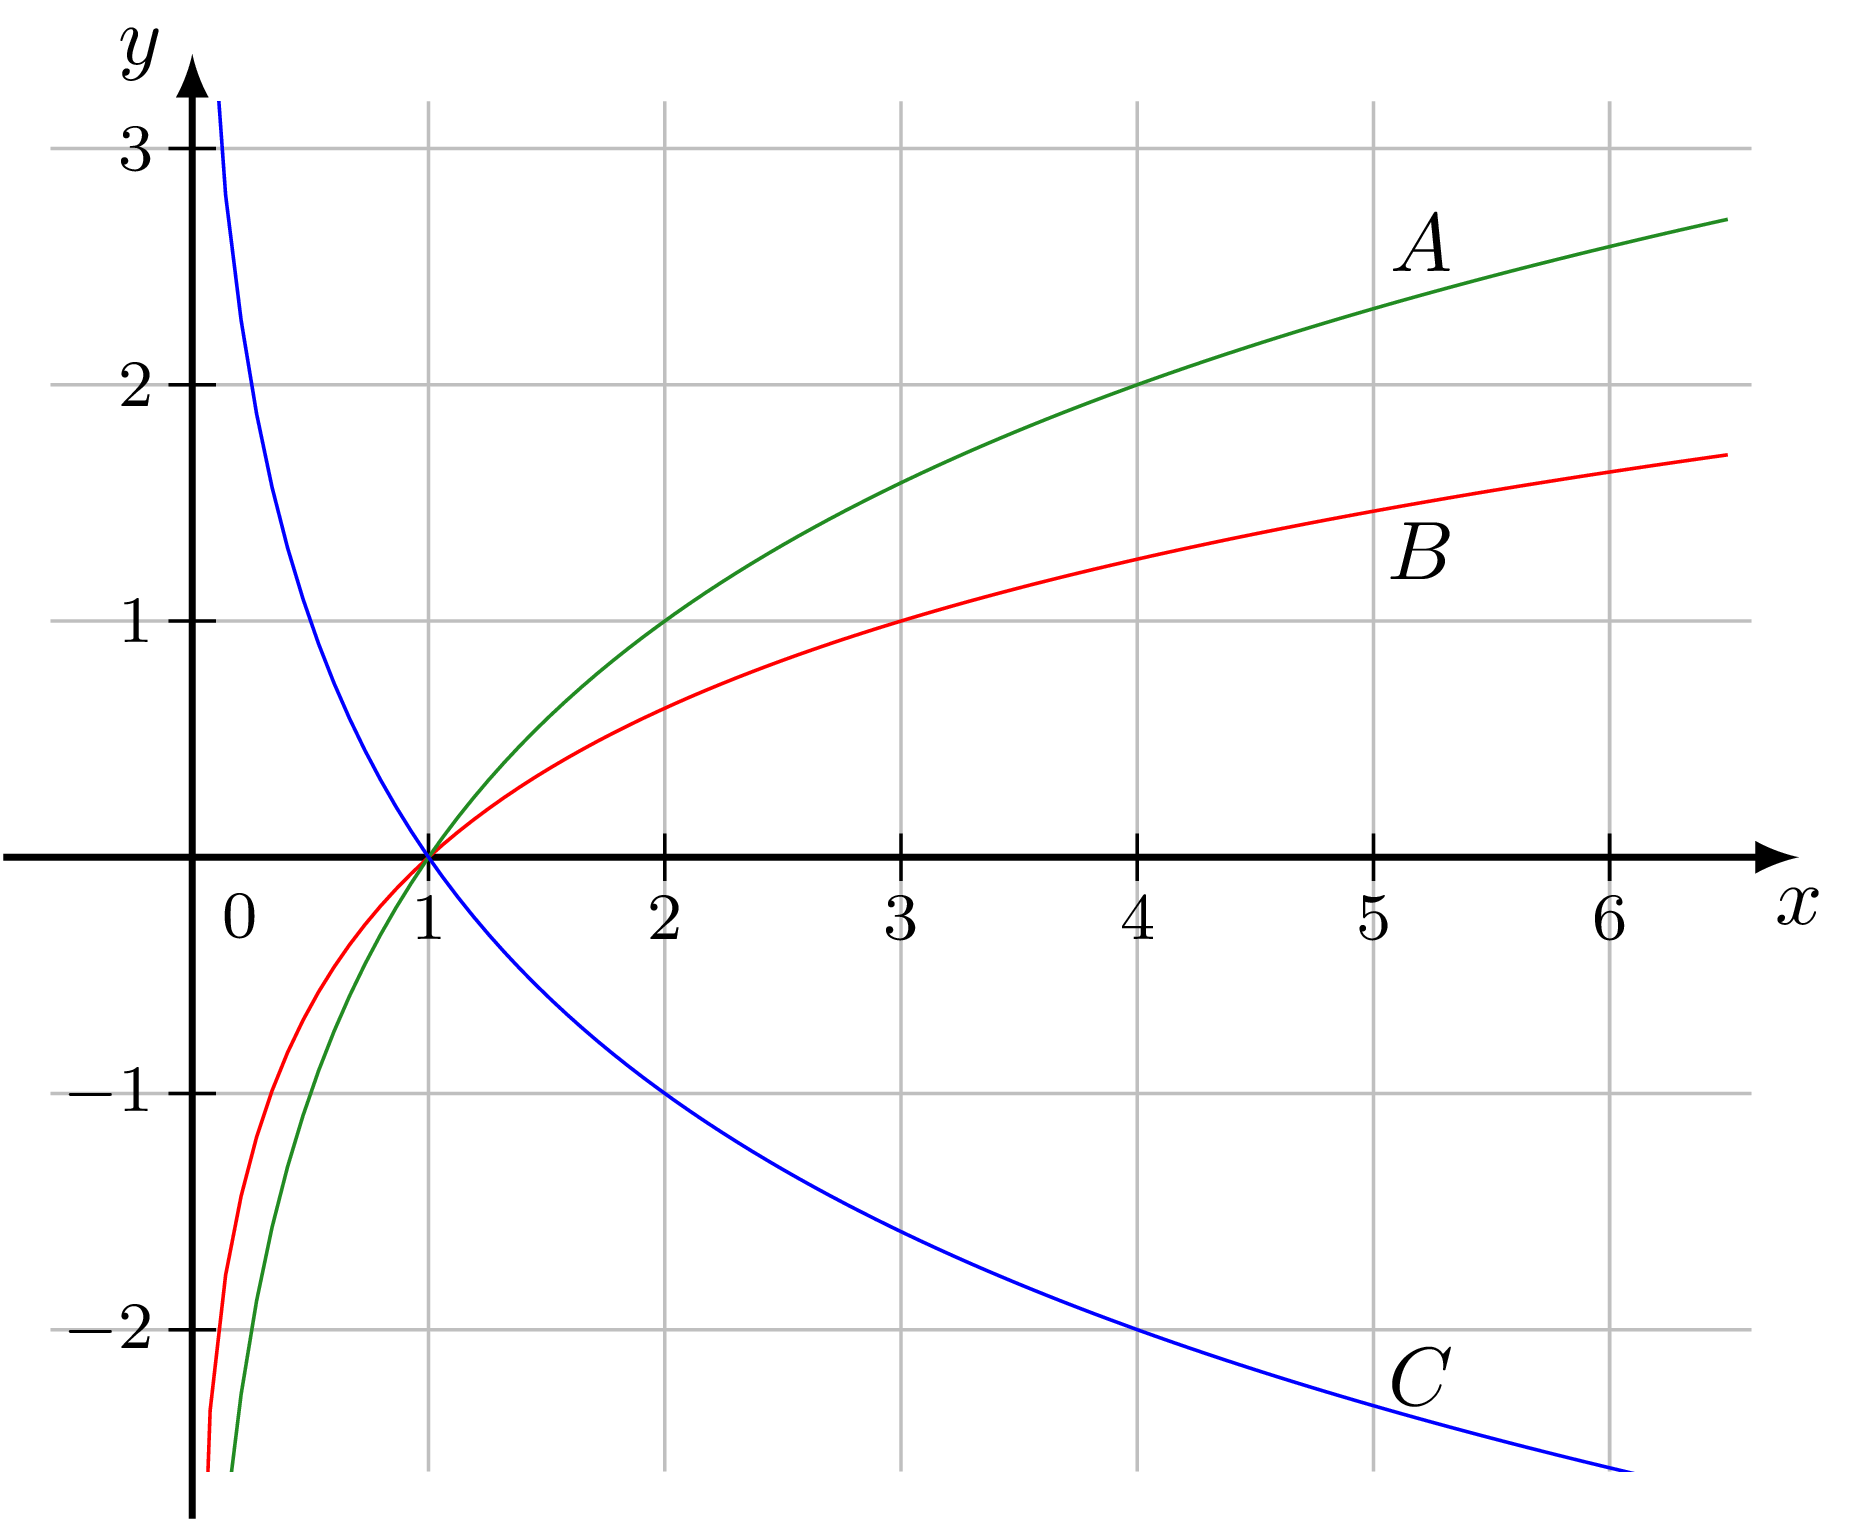
\includegraphics[scale=0.08]{data-algebra/LogGraph.png}
\end{minipage}

%---------------------------------------------------------
\noaddpoints
\question[\totalpoints]
\addpoints
\begin{minipage}{0.6\linewidth}
    \begin{parts}
        \part[2] Gezeichnet sind drei Graphen von Funktionen der Form $y=\Log{b}{x}$. Gib an welcher zur Funktion mit der kleinsten und welcher zur Funktion mit der grössten Basis $b$ gehört.
        \part[1] Gib die Basis der Funktion des Graphen $\textcolor{forestgreen}{A}$ an.
    \end{parts}
\end{minipage}
\hfill
\begin{minipage}{0.35\linewidth}
    \centering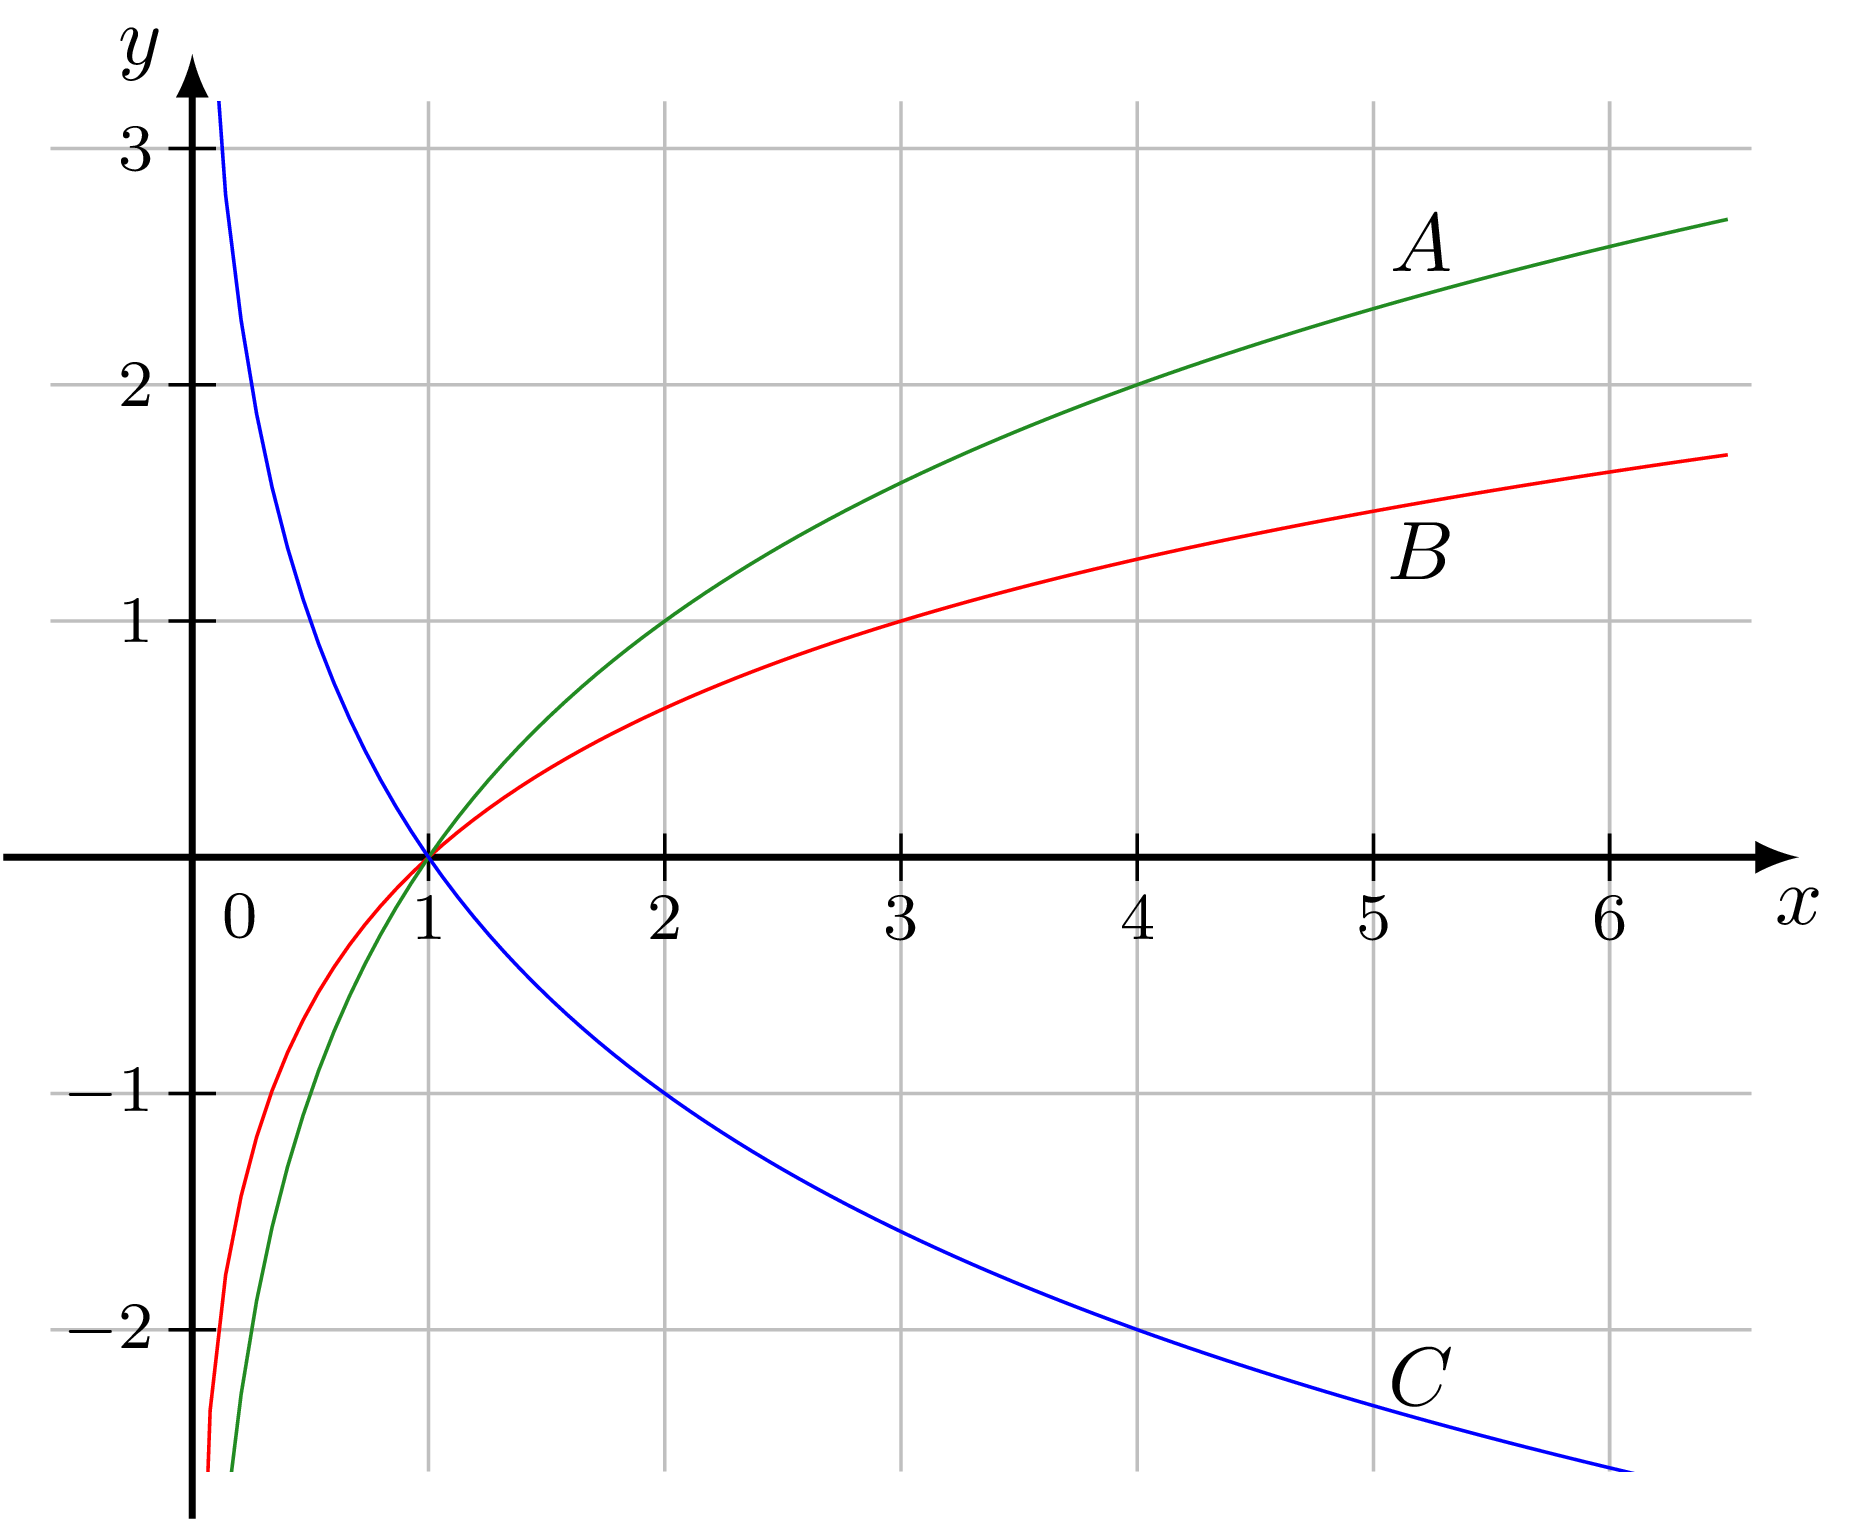
\includegraphics[scale=0.08]{data-algebra/LogGraph.png}
\end{minipage}

%---------------------------------------------------------
\question[3]
\begin{minipage}{0.55\linewidth}
    Im Koordinatensystem sind drei Graphen von Logarithmusfunktionen der Form $f(x)=\Log{a}{x}$ eingezeichnet. Gib die drei Funktionsgleichungen an.
\end{minipage}
\hfill
\begin{minipage}{0.4\linewidth}
    \centering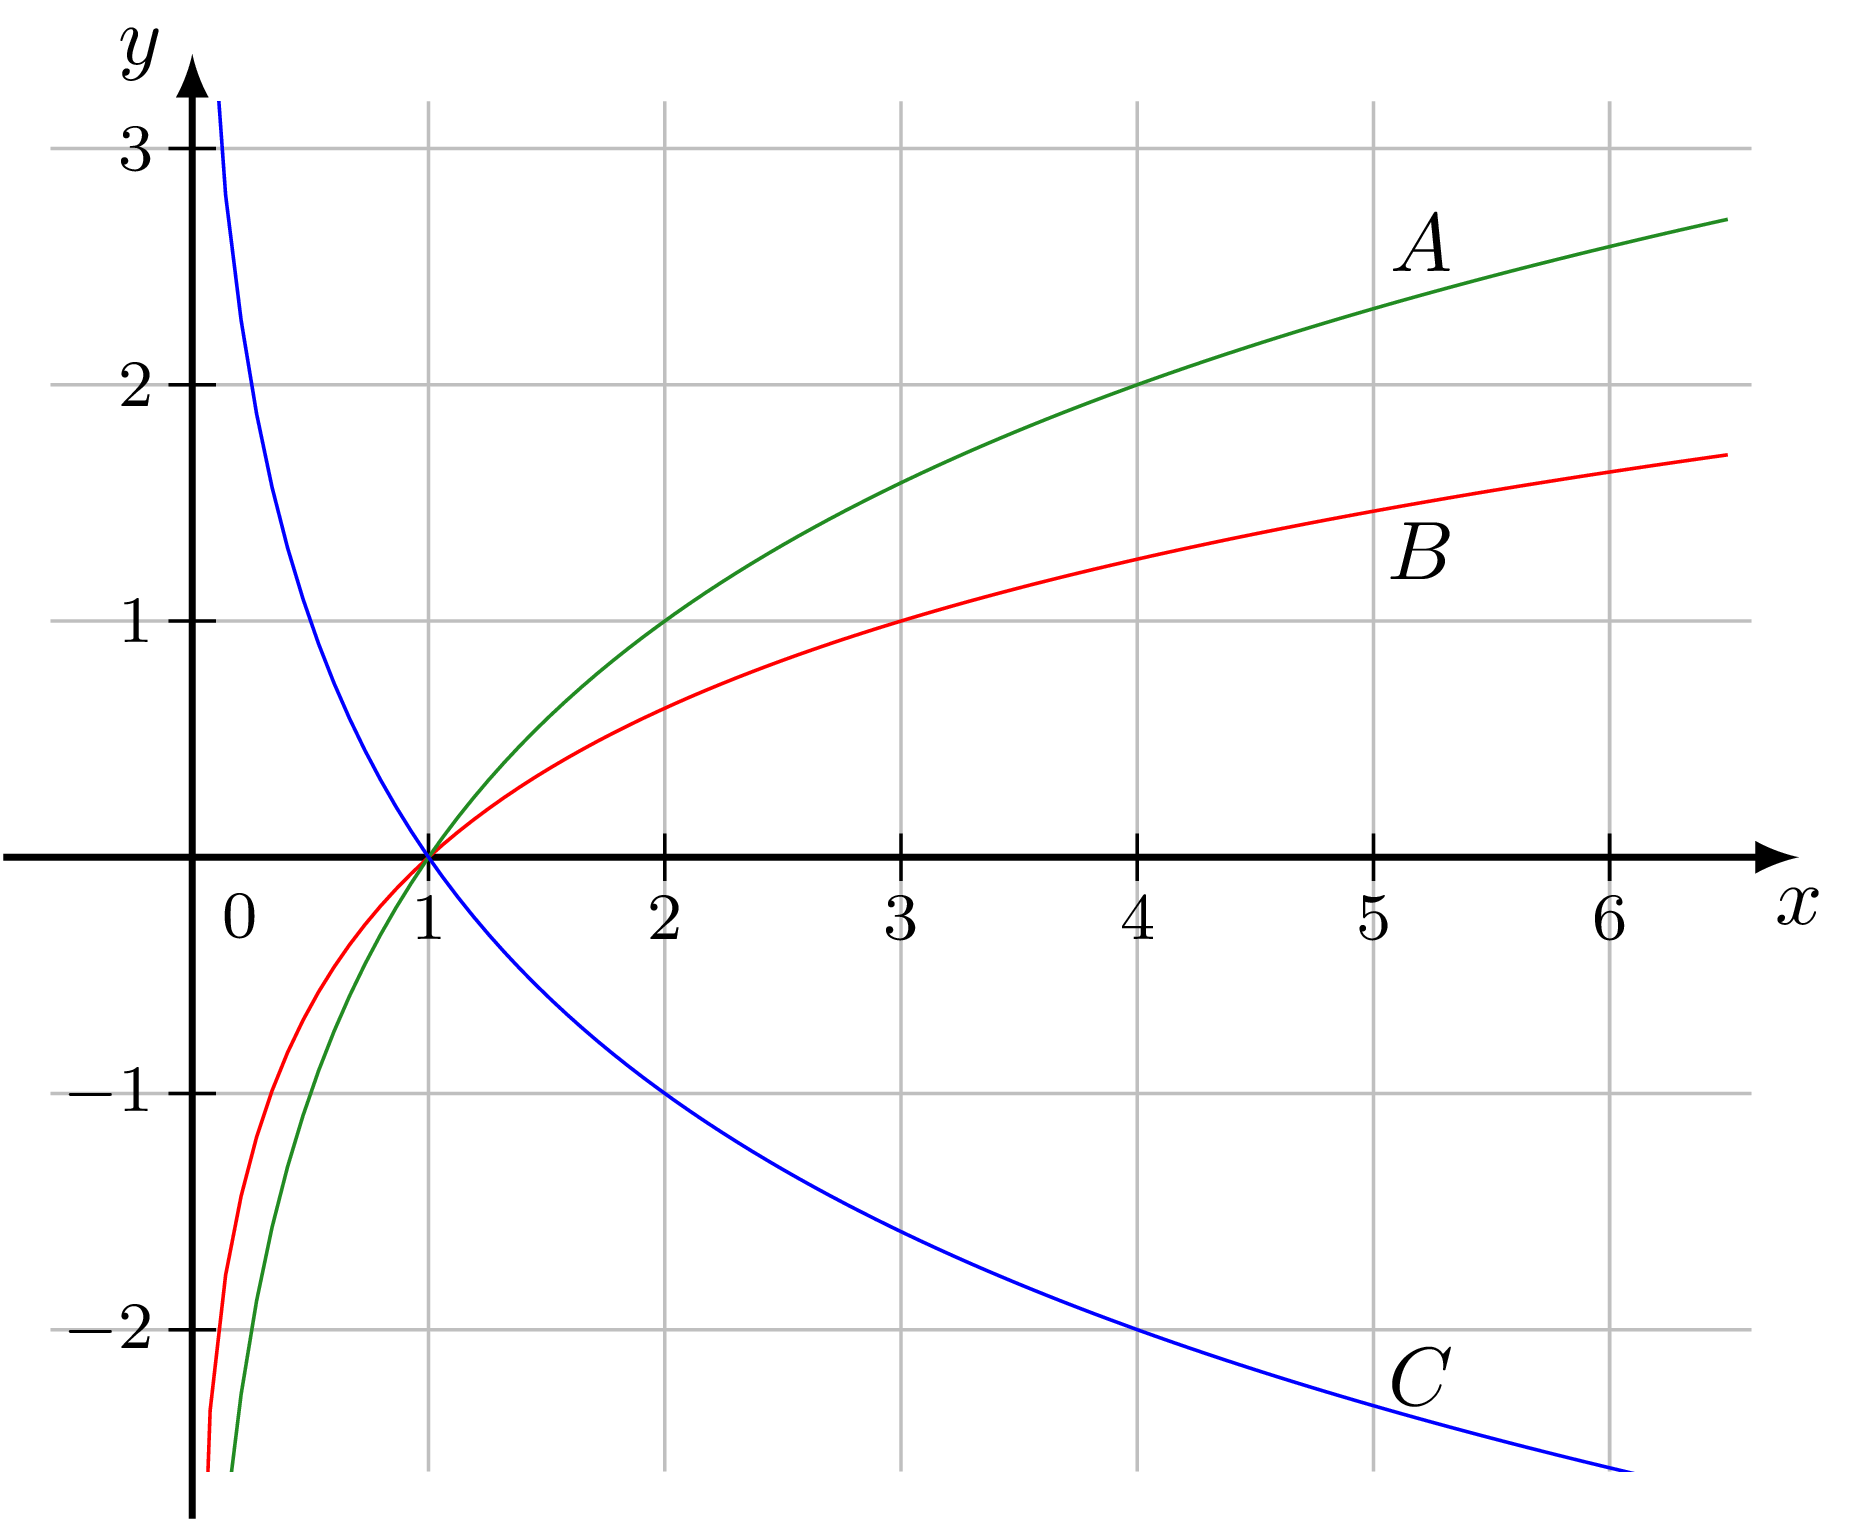
\includegraphics[scale=0.1]{data-algebra/LogGraph.png}
\end{minipage}

%---------------------------------------------------------
\noaddpoints
\question[\totalpoints]
\addpoints
Salmonellen sind Bakterien, die schwere Magen-Darm Erkrankungen auslösen. Bei Temperaturen von über $8^\circ$C vermehren sich Salmonellen exponentiell. Die infektiöse Dosis beträgt ca. eine Million Keime.\newline Bei einem infizierten Ei werden um 10:00 Uhr $1000$ Keime gezählt, um 12:00 Uhr sind es bereits $5500$.
\begin{parts}
    \part[1] Gib eine Funktion an, mit welcher sich die Anzahl Keime nach $t$ Stunden ausgehend von 10:00 Uhr berechnen lässt.
    \part[1] Bestimme die Zeit, in der sich die Keimzahl verdoppelt?
    \part[3] Um 16:00 Uhr wird das Ei in ein Kühlfach mit $12^\circ$C gelegt. Das bewirkt, dass sich die Verdopplungszeit\footnote{Die Verdopplungszeit bezeichnet die Zeitspanne, nach der sich der Bestand einer exponentiell wachsende Grösse verdoppelt hat.} vervierfacht. Berechne, um welche Uhrzeit die infektiöse Dosis an Keimen erreicht ist.
\end{parts}

%---------------------------------------------------------
\question[4]
Löse die folgende Gleichung ohne Verwendung von \flqq solve\frqq\:nach $x$ auf. \[\Log{2}{x}=1+\Log{4}{x}\]
\begin{small}
    Bewertung: Lösungen ohne Lösungsweg ergeben keine Punkte.
\end{small}

%---------------------------------------------------------
\question[4]
Löse die folgende Gleichung ohne Verwendung von \flqq solve\frqq\: nach $x$ auf. \[\Log{3}{x-2}=\Log{9}{x}\]
\begin{small}
    Bewertung: Lösungen ohne Lösungsweg ergeben keine Punkte.
\end{small}

%---------------------------------------------------------
\question[4]
Löse die folgende Gleichung ohne Verwendung des Taschenrechners nach $x$ auf. \[\Log{x}{7x-10}=2\]
\begin{small}
    Bewertung: Lösungen ohne Lösungsweg ergeben keine Punkte.
\end{small}


%---------------------------------------------------------
\question[2]
Entscheide in der Tabelle unten, ob die Aussagen wahr oder falsch sind. Die Antworten müssen nicht begründet werden.\newline
\begin{small}
    Bewertung: Für $0-2$ korrekte Antworten gibt es keine Punkte; $3$ korrekte Antworten einen Punkt und falls alle Antworten korrekt sind, gibt es $2$ Punkte.
\end{small}
\begin{table}[h]
    \centering
    \begin{tabular}{|p{12cm}|c|c|}\hline
         & wahr & falsch \\\hline
        Der Logarithmus ist eine alternative Darstellung eines Exponent. & & \\\hline
        Polynomialgleichungen können mithilfe des Logarithmus gelöst werden. & & \\\hline
        Durch geeignetes Logarithmieren kann eine Multiplikation in eine Summe vereinfacht werden. & & \\\hline
        Die Definitions- und Wertemenge sind für die Exponentialfunktion und die Logarithmusfunktion exakt die Gleichen. & & \\\hline
        Durch geeignetes Logarithmieren kann eine Multiplikation in eine Division vereinfacht werden. & & \\\hline
        Exponentialgleichungen können mithilfe des Logarithmus gelöst werden. & & \\\hline
        Der Logarithmus ist eine alternative Darstellung eines Potenz. & & \\\hline
    \end{tabular}
\end{table}


\end{questions}
\end{document}